\documentclass[12pt,a4paper,twosided]{article}
\usepackage{amsmath,bm} 
%\usepackage[T1]{fontenc}
%\usepackage[QX]{fontenc}
%\usepackage[normalsections]{savetrees}
\usepackage{tgschola}
\usepackage[latin1]{inputenc}
\usepackage{paralist}
\usepackage{enumitem}
\usepackage{graphicx}
\usepackage{xcolor}
\usepackage{xspace}
\usepackage{booktabs}
\usepackage{listings}
\usepackage[per=frac,fraction=nice]{siunitx}
\usepackage[colorlinks=true,linkcolor=black,urlcolor=black,hyperfootnotes=false]{hyperref}
\pdfpagewidth=210mm
\pdfpageheight=297mm
% +++++++++++++++++++++++++++++++++++++++++++
\newcommand{\wnat}{\omega_\text{n}}
\newcommand{\fmax}{f_\text{max}}
\newenvironment{enumin}%
% {\begin{inparaenum}[\hspace{1em}(1)]\hspace{-1em}\ignorespaces}%
   {\begin{inparaenum}[\hspace{0.6em}(1)]}%
   {\end{inparaenum}}
%%%
\graphicspath{{xfig/}}
\title{Dynamics of Structures 2010-2011\\\large 1st home assignment
  due on Tuesday 2011-06-17\\\huge Solutions}
\date{}
\setcounter{tocdepth}{1}
%%%
\begin{document}
\lstset{
  basicstyle=\ttfamily\small,
  backgroundcolor=\color[rgb]{1.00,0.98,0.95},
  language=python,
  showstringspaces= false
}
\maketitle{}
\tableofcontents{}
% +++++++++++++++++++++++++++++++++++++++++++
\section{Impact}
\[\input{xfig/impact.pdf_t}\]
\noindent A body of mass $m_1=\SI{120}{\kilogram}$ hits an undamped
\emph{SDOF} system, of unknown characteristics $k$ and $m_2$, with
velocity $\dot{x}_1=\SI{50}{\meter\per\second}$.

The collision is anelastic, i.e., the two masses are \emph{glued} together
and a measurement of the ensuing free oscillations gives the following
results:
\[ x_\text{max} =\SI{30}{\milli\meter},\qquad
   \dot{x}_\text{max}=\SI{60}{\milli\meter\per\second}.\]
%
Compute:
\begin{enumerate}
\item the total mass $m=m_1+m_2$
\item the mass $m_2$ of the impacted body,
\item the circular frequency of the insuing motion,
\item the spring stiffness $k$.
\end{enumerate}

\subsection{Solution}

After the collision the two \emph{glued} bodies have the same
velocity, so that by the law of conservation of the momentum we can
write
\[m_1\times\dot x_1 + m_2\times0 = (m_1+m_2)\times\dot x_0,\]
where we have denoted the initial velocity of the compound body with
$\dot x_0$. 

Observing that the initial conditions for the compound are $x(0)=0$
and $\dot x(0)=\dot x_0$ we can write
\begin{align*}
  x(t)&=\frac{\dot x_0}{\wnat}\,\sin\wnat t,\,&\dot x(t)&=\dot x_0\,\cos\wnat t.\\
  x_\text{max} &= \frac{\dot x_0}{\wnat} = \SI{30}{\mm},&
  \dot x_\text{max} &=\dot x_0=\SI{60}{\milli\meter\per\second}\\
  \intertext{and hence}
  \dot x_0&=\SI{60}{\milli\meter\per\second},&
  \wnat&=\frac{\dot x_\text{max}}{x_\text{max}}={\color{red}\SI{2}{\rad\per\second}}.
\end{align*}

Substituting $\dot x_0=\SI{60}{\mm\per\second}$ in
$m_1\times\dot x_1 + m_2\times0 = (m_1+m_2)\times\dot x_0$ we have
\[\SI{120}{\kg}\times\SI{50000}{\mm\per\second} = 
(\SI{120}{\kg}+m_2)\times\SI{60}{\mm\per\second}
\Rightarrow {\color{red}m=\SI{100000}\kg}
\Rightarrow {\color{red}m_2=\SI{99880}\kg}.\]

As for the last question, it is $k=\wnat^2\,m$ and substituting we find
\[{\color{red}k=(\SI{2}{\rad\per\second})^2\,\SI{100000}{\kg}=\SI{400000}{\newton\per\meter}.}\]
\section{Vibration Isolation --- Numerical Integration} 
A rotating machine, its mass $M=\SI{35000}{\kg}$, is rigidly connected
to the floor.

Due to unbalances, during steady-state regime the machine is subjected
to a harmonic force $p(t)=\SI{1}{\kilo\newton}\,\sin(2\pi\,\SI{5}\hertz\, t)$.

\subsection{Vibration Isolation}
Considering the floor fixed, design an appropriate suspension system
such that the steady-state transmitted force is reduced to 
\SI{300}{\newton}.
\subsection{Numerical Integration}
When the machine is turned on, its full velocity is reached in
\SI{6}{\second}.  The angular velocity and the unbalanced load vary
linearly, from $0$ to their respective maximum values, i.e.,
\[p(t)=
\begin{cases}
  \SI{1}{\kilo\newton}\,\frac{t}{\SI{6}\second}\;
  \sin\left(2\pi\,\SI{2.5}{\hertz}\,\frac{t^2}{\SI{6}{\second}}\right) &  \SI{0}\second \le t \le \SI{6}\second,\\
  \SI{1}{\kilo\newton}\;\sin(2\pi\,\SI{5}{\hertz}\, t) &  \SI{6}\second\le t.
\end{cases}\]\[
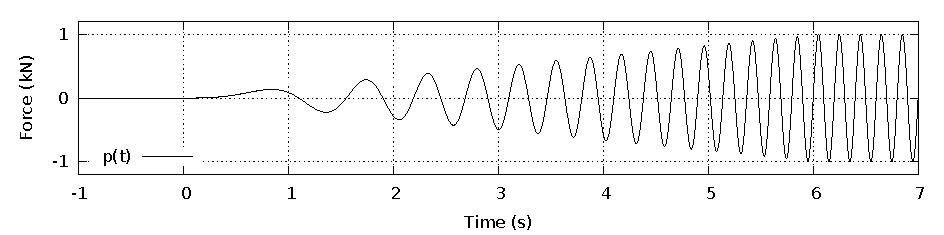
\includegraphics{02/p_of_t}
\]

\bigskip\noindent Using the stiffness computed in the previous step,
find  the maximum absolute value of the displacement using either
the constant or the linear acceleration method and plot the response
in the interval $\SI{0}\second \le t \le \SI{10}\second$.

\subsection{Solution}
\subsubsection{Vibration Isolation}
With $\wnat$ being the natural frequency of the system composed by the
machine and the suspension springs, $\beta=\frac\omega\wnat$ the
frequency ratio, the condition on the maximum tranmitted load is
\[\fmax=\frac{p_0}{\beta^2-1}\le\SI{300}{\newton}.\]

Substituting $p_0=\SI{1000}{\newton}$ in the equation above, we have 
\[ \beta^2 =\frac{\omega^2}{k/m} \ge \frac{13}{3}
\quad\Rightarrow\quad
k\le\frac{3}{13}(\pi\,\SI{10}{\rad\per\second})^2\SI{35000}\kg=\SI{7971603.}{\newton\per\metre}\]

If we accept a small damping, it must be
\[\text{TR} =
\frac{\sqrt{1^2+(2\beta\zeta)^2}}{\sqrt{(1-\beta^2)^2+(2\beta\zeta)^2}}
=
\frac{\sqrt{1+4\beta^2\zeta^2}}{\sqrt{(1-\beta^2)^2+4\beta^2\zeta^2}}\le0.4\]
with $\omega=2\pi\SI{5}{\rad\per\second}$ and $\wnat^2=k/m$,
substituting the actual value of $m$, solving the quadratic equation
in $k$ and discarding the negative root, it is finally found
\[k\le \left( \sqrt{\left(182 \zeta^2 + 9\right)^2 + 819} - \left(182
    \zeta^2 + 9\right) \right) \frac{\pi^2}
{26}\si{\mega\newton\per\metre}\]
\[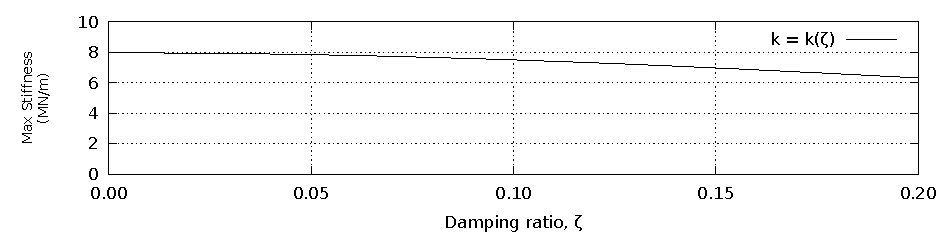
\includegraphics{02/stif_from_z}\]

\subsubsection{Numerical Integration}
The response can be computed and printed with the following program
\lstinputlisting{02/integ.py}
and the response time history is
\[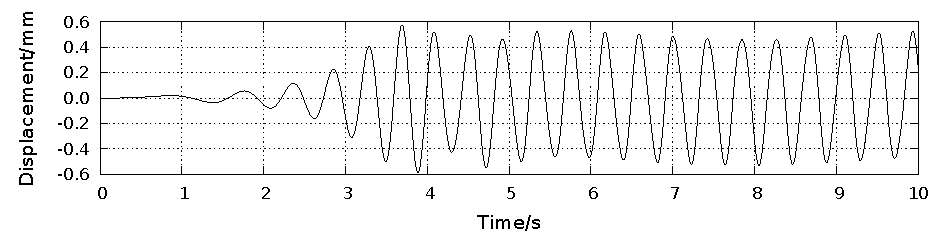
\includegraphics{02/displacement}\]
but these displacements are a bit meaningless, let's try to plot
$f_\text{S}=k\,x$
\[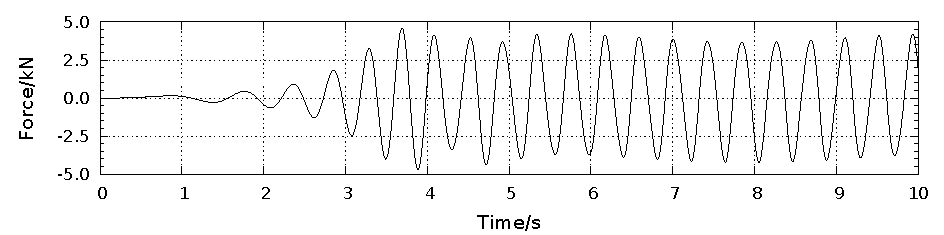
\includegraphics{02/force}\]
oh my, it's $f_\text{S}\approx\SI{5}{\kilo\newton}$! just a moment,
the machine weight is about \SI{350}{\kilo\newton} so this harmonic
force is less than 1/70 of the weight, it shouldn't be a structural
problem... on the other hand, there is no dissipation and the effects
of the transient become permanent, it should be obvious that we have to
use a dissipative device.

To get an appreciation of the problem, I have  modified the previous
program so that the integration is run for different values of $t_0$,
the duration of transient, and different values of the damping ratio
$\zeta$; for each value of $\zeta$ $k$ is given by the formula we have
seen before, 
\[k\le \left( \sqrt{\left(182 \zeta^2 + 9\right)^2 + 819} - \left(182 \zeta^2 + 9\right) \right) \frac{\pi^2} {26}\si{\mega\newton\per\metre}\]
and the damping coefficient is computed by
\[\wnat=\sqrt{k/m},\qquad c=2\zeta\wnat m.\]

For each iteration on $\zeta,\;t_0$ the program prints the peak value
of the transmitted force, and finally the results are plotted as a
colour map
\[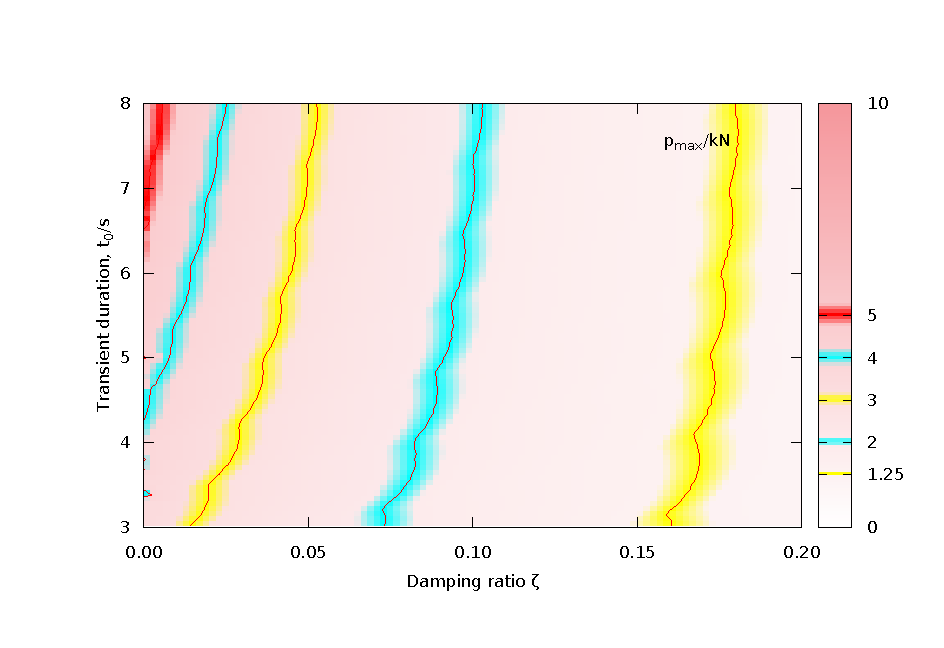
\includegraphics{02/map}\]
% +++++++++++++++++++++++++++++++++++++++++++
%
\section{Estimation of damping ratio}
You want to determine the mass $m$, the stiffness $k$ and the damping
ratio $\zeta$ of a one storey building that can be modeled as a single
degree of freedom system.

A series of 4 dynamical test is performed, loading the building with a
vibrodyne and measuring the amplitude $\rho$ and the phase difference
$\theta$ of the steady state motion (note that the measures of $\rho$
and $\theta$ are affected by a random measurement error).

In each test the load amplitude is $p_0=\SI{600}{\newton}$, while
the excitation frequencies $\omega_n$ (with $n=1,\ldots,4$) are
different.

The relevant data is summarized in the following table
\begin{center}
  \begin{tabular}{rcrr}
    \toprule 
    $n$ & 
    $\omega_n (\si{\rad\per\second})$ & 
    $\rho_n (\si{\micro\metre})$  &
    $\theta_n (\si{\deg})$\\
    \midrule
    1 & 40 & 12.39062 &   7.58258 \\
    2 & 50 & 41.09556 &  33.33505 \\
    3 & 60 & 18.07490 & 163.21210 \\
    4 & 70 &  7.11246 & 171.69968 \\
    \bottomrule
  \end{tabular}
\end{center}
Give your best estimate of $m$, $\zeta$ and $k$.

\subsection{Solution}

When you have a linear system $\bm A\,\bm x=\bm b$ with more equations
than unknowns, it is usually solved under the hypotesis that the
\emph{best} solution is the solution that minimises the sum of the
squares of the residuals $\bm r = \bm b - \bm A\,\bm x$. In a vector
notation, the sum of the
squares of the residuals is
\begin{align*}
  \bm r^T\cdot\bm r & = (\bm b^T - \bm x^T \bm A^T)(\bm b - \bm A\,\bm x )\\
  &=\bm b^T\bm b+ \bm x^T\bm A^T\bm A\,\bm x -\bm x^T \bm  A^T\bm b -\bm b^T\bm A\,\bm x\\
\intertext{the last term is the transpose of the previous one, both
  are scalars, so we can write}
  \bm r^T\cdot\bm r &=\bm b^T\bm b+ \bm x^T\bm A^T\bm A\,\bm x -2\bm x^T \bm  A^T\bm b.
\end{align*}

The square of the residual is positive definite, and its minimum is
achieved when all the partial derivatives with respect to the $x_i$
are equal to zero,
\[\frac{\partial (\bm r^T\cdot\bm r)}{\partial x_i}=0,\qquad
i=1,\ldots,N.\]

These $N$ equations can be conveniently be expressed in matrix format,
\[2(\bm A^T\bm A\,\bm x - \bm A^T  \bm b)=0\quad\Rightarrow\quad \bm
A^T\bm A\,\bm x = \bm A^T  \bm b.\]

In our case, it is
\[1\cdot k - \omega^2_n\,m=p_0\frac{\cos\theta_n}{\rho_n},\qquad
n=1,\ldots,4\]
or, matricially
\[
\begin{bmatrix}  1&-1600\\1&-2500\\1&-3600\\1&-4900\end{bmatrix}\,
\begin{Bmatrix}k\\m\end{Bmatrix}=
\begin{Bmatrix} +48.000\\+12.198\\-31.780\\-83.475\end{Bmatrix}\,\si{\mega\newton\per\metre}
\]
(note that the coefficients of $m$ are, dimensionally, a square
frequency) premultiplying both members by the transpose of the
coefficient matrix we write
\[\left\{
  \begin{matrix}
    +4 \cdot k & -\SI{2600}{\per\second\squared} \cdot m &=&
    \SI{-55.058e6}{\newton\per\metre}\\
     - \SI{2600}\cdot k &+ \SI{45780000}{\per\second\squared} \cdot m &=&\SI[retainplus]{+416.14e+9}{\newton\per\metre}
  \end{matrix}
\right.,\]
where the second equation was multiplied by \si{\second\squared}.

Solving the previos linear system gives the best estimates
${\color{red}k=\SI{111.78e6}{\newton\per\metre}}$ and
${\color{red}m={39854}{\kg}}$, in good agrement with the data entered in
the simulation. The damping ratio, computations omitted, is
${\color{red}\zeta\approx3.8\%}$.
% +++++++++++++++++++++++++++++++++++++++++++
\section{Generalised Coordinates (rigid bodies)}

%\[\resizebox{0.8\textwidth}{!}{\input{xfig/newtrab.pdf_t}}\]
\[\input{xfig/newtrab.pdf_t}\]

\renewcommand{\ss}{\textsf}
\noindent The articulated system in figure, composed by
\begin{itemize}
\item two rigid bars, \begin{enumin}\item \textsf{ABC} and
  \item\textsf{CDE},
  \end{enumin}
\item three fixed constraints,
  \begin{enumin}
  \item a horizontal roller in \textsf{A},
  \item an internal hinge in \textsf{C} and
  \item a hinge in \textsf{E},
  \end{enumin}
\item two deformable constraints,
  \begin{enumin}
  \item a horizontal spring in \textsf{A}, its stiffness${}=k$ and
  \item a vertical dashpot in \textsf{C}, its damping
    coefficient${}=c$,
  \end{enumin}
\end{itemize}
is excited by a horizontal harmonic  force applied in \textsf{B},
\(p(t)=p_0\,\sin\omega t.\)

The vertical parts of the two bars, \textsf{AB} and \textsf{ED}, are
massless while both the horizontal parts, \textsf{BC} and \textsf{CD},
have a constant unit mass $\overline m$, with $\overline m\,L=m$.

\medskip\noindent Using $u_\textsf{A}$ (the horizontal displacement of
\textsf{A}) as the generalised coordinate
\begin{enumerate}
\item compute the generalised parameters $m^*$,  $c^*$ and $k^*$,
\item compute the generalised loading $p^*(t)$ and
\item write the equation of dynamic equilibrium.
\end{enumerate}
\subsection{Solution}
Our sistem of reference will be centred in \textsf A, so that the
positions of the Center of Instantaneous Rotation (CIR) for the two
rigid bodies are $\Omega_1=(0,3L)$ and
$\Omega_2=(3L,0)\equiv\textsf{E}$. Using $Z=u_\ss A$ as our free
coordinate, the rotation about $\Omega_1$ is $\theta_1=+1/3\,Z/L$, the
rotation about $\Omega_2$ is $\theta_2=-2/3\,Z/L$ (anticlockwise
rotations are positive), and then we can compute the relevant
displacements

\medskip
\centerline{\begin{tabular}{ccc}
  \toprule
  & $u/Z$ & $v/Z$\\
  \midrule
  \ss A           & 1 & 0\\
  \ss B           & 2/3 & 0\\
  \ss C           & 2/3 & 2/3\\
  $\ss G_1$  & 2/3 & 1/3\\
  $\ss G_2$  & 2/3 & 1/3\\
  \bottomrule
\end{tabular}}

\medskip For equilibrium, the external virtual work $\delta W_\text E$ (work of
the external, spring, damper and inertial forces) equals to the
internal virtual work, $\delta W_\text I$ but for a rigid system it is
$\delta W_\text I = 0$, hence our equilibrium equation is
\[\delta W_\text E = 0.\]

In detail,
\begin{multline*}
  p(t)\,\frac23\delta Z + (-kZ)\,\delta Z + (-c\frac23\dot Z)\,(\frac23\delta Z) +\\
  (-(2m)\frac23\ddot Z)\,(\frac23\delta Z) + (-(2m)\frac13\ddot Z)\,(\frac13\delta Z) +
  (-\frac{2m(2L)^2}{12}\frac{\ddot Z}{3L})\,(\frac{1}{3L}\delta Z) +\\
  (-m\frac23\ddot Z)\,(\frac23\delta Z) + (-m\frac13\ddot Z)\,(\frac13\delta Z) +
  (\frac{mL^2}{12}\frac{2\ddot Z}{3L})\,(-\frac2{3L}\delta Z) = 0
\end{multline*}
simplyfying $\delta Z$, collecting $Z$ and its derivatives, moving
$Z$'s on the right side of the equation, it is
\begin{align*}
  \frac23 p(t) &= k\,Z + \frac49c\,\dot Z + (\frac89+\frac29+\frac2{27}+\frac49+\frac19+\frac1{27})m\,\ddot Z\\
               &= \frac{16}9m\,\ddot Z + \frac49c\,\dot Z + k\,Z
\end{align*}

The required answers are 
\[\color{red}
m^*=\frac{16}9m,\quad c^*=\frac49c,\quad k^*=k,\quad p^*=\frac23p(t),
\] and
\[\color{red} \frac{16}9m\,\ddot Z + \frac49c\,\dot Z + k\,Z =
\frac23p(t)\]
% +++++++++++++++++++++++++++++++++++++++++++
\section{Rayleigh quotient}
\label{sec:rayleigh}
\[\input{xfig/newtrab2.pdf_t}\]
\noindent The undamped 3 \emph{DOF} system in figure is composed of 3
identical rigid bars, their masses $m_i=m$, and three vertical
springs, their stiffnesses as detailed in figure.  Starting with a
trial shape $\bm{\phi}= \begin{Bmatrix} 1 & 1 & 1
\end{Bmatrix}^T$ so that $u_1=u_2=u_3=Z_0\,\sin\omega t$, give the successive
Rayleigh estimates of (squared) free vibration circular frequency
$R_{00}$, $R_{01}$ and $R_{11}$. 

Note
\begin{enumin}
\item that the bars have a not negligible rotatory inertia:
  $J_i=mL^2/12$, that you must take into account and
\item that the free coordinates are not referred to the centres of
  mass of the bars (hence a non-diagonal mass matrix).
\end{enumin}

\smallskip\noindent\textsc{Hint:} {\small
 %
  the nodal inertial forces are $\bm f_\text{I}=\bm M\,\ddot{\bm u}$,
  the mass matrix's coefficients can be deduced comparing an explicit
  derivation of the kinetic energy $T$ in terms of the velocities
  $\dot u_i$, the mass $m$ and the inertia $J$ to the matrix
  expression $T=\frac12 \dot{\bm u}^T \bm M\,\dot{\bm u} = \frac12
  \left( m_{11}\, \dot x_1^2 +\cdots+(m_{12}+m_{21})\,\dot x_1 \dot x_2 +
    \cdots \right)$, where $m_{ij}=m_{ji}$.}

\subsection{Solution}

The displacements $x_i$ of the 3 centres of mass are 
\begin{align*}
  x_1&=u_1/2,      &x_2&=(u_2+u_1)/2&x_3&=(u_3+u_2)/2),\\
  \intertext{the rotations $\theta_i$ are}
  \theta_1&=u_1/L, &\theta_2&=(x_2-x_1)/L&\theta_3&=(x_3-x_2)/L. 
\end{align*}

The kinetic energy is, summing the contributions from the three
identical bars,
\begin{align*}
  T&=\frac12\left(m(\dot x_1^2 + \dot x_2^2 + \dot
    x_3^2)+\frac{mL^2}{12}(\dot\theta_1^2 + \dot\theta_2^2 +
    \dot\theta_3^2)\right).\\
  \intertext{Substituting the free coordinates, simplifying and
    collecting the similar terms, it is}
  T&=\frac12\,\left(8\,\dot u_1^2 + 8\,\dot u_2^2 + 4\,\dot u_3^2 +
    4\, \dot u_1 \dot u_2 + 4\, \dot u_2 \dot u_3 + 0\, \dot u_3 \dot
    u_1\right)\,\frac m{12}.
\end{align*}

The kinetic energy can be expressed also by a matrix product,
\[T=\frac12\,\bm u^T\bm M\,\bm u=\frac12\left(m_{11}\dot u_1^2
  +\cdots+2\,m_{12}\dot u_1 \dot u_2 + \cdots\right),\]

equating the two right members term by term, we deduce that the mass
matrix coefficients are as in
\[\bm M =\frac m6 \begin{bmatrix}  4&1&0\\1&4&1\\0&1&2 \end{bmatrix}.\]

The stiffness matrix, simply, is
\[\bm K = k \begin{bmatrix} 1&0&0\\0&2&0\\0&0&3 \end{bmatrix}.\]

The Rayleigh procedure starts writing
\begin{align*}
  \bm{u}(t)&=\bm{\phi} Z_0 \sin\omega t,&\dot{\bm u}(t)&=\omega\bm\phi Z_0 \cos\omega t,\\
  V&=\frac12\bm\phi^T\bm{K}\,\bm\phi\,Z_0^2\sin^2\omega{}t,&
  T&=\frac12\omega^2\bm\phi^T\bm{M}\,\bm\phi\,Z_0^2\cos^2\omega{}t,
\end{align*}
so that, by equating the maximum values of energies $V$ and $T$ and
substituting $\bm\phi=\begin{Bmatrix}1&1&1\end{Bmatrix}^T$ we have
\[\omega^2=\frac{\bm\phi^T\bm{K}\,\bm\phi}{\bm\phi^T\bm{M}\,\bm\phi}=\frac{6k}{7/3\;m}=\frac{18}7\frac
km=\color{red}2.5714\frac km.\]

A better approximation of the strain energy is given by
\[V=\frac12\bm{u}_\text{I}^T\bm{f}_\text{I}^{},\] where
\(\bm{f}_\text{I}=-\omega^2\bm{M}\bm{\phi}Z_0\sin\omega{t}\) is the
vector of the inertial forces and
\(\bm{u}_\text{I}=\bm{K}^{-1}\bm{f}_\text{I}=-\omega^2\bm{K}^{-1}\bm{M}\bm{\phi}Z_0\sin\omega{t}\)
is the vector of displacements produced by $\bm{f}\text{I}$.

Equating the new maximum value of the strain energy to the old kinetic
energy maximum, it is
\[\omega^2=\frac{\bm\phi^T\bm{M}\,\bm\phi}{\bm\phi^T\bm{M}\,\bm{K}^{-1}\bm{M}\bm\phi}=
\frac{7/3\;m}{23/18\;m^2/k}=\frac{42}{23}\frac
km=\color{red}1.8261\frac km.\]

A better approximation to the kinetic energy is given by
\[T=\frac12 \dot{\bm{u}}_\text{I}^T\bm{M}\,\dot{\bm{u}}_\text{I},\]
where \(\dot{\bm{u}}_\text{I}=-\omega^3\bm{K}^{-1}\bm{M}\bm{\phi}Z_0\cos\omega{t}\)
is the velocity due to  application of the inertial
forces, equating the new max of $T$ to the new max of $V$ we have
\[\omega^2=\frac{\bm\phi^T\bm{M}\,\bm{K}^{-1}\bm{M}\bm\phi}{\bm\phi^T\bm{M}\,\bm{K}^{-1}\bm{M}\,\bm{K}^{-1}\bm{M}\bm\phi}
  =\frac{23/18\;m^2/k}{29/36\;m^3/k^2}=\frac{46}{29}\frac
  km=\color{red}1.5862\frac km.\]
% +++++++++++++++++++++++++++++++++++++++++++
\section{3 DOF System}
With reference to the system of problem \ref{sec:rayleigh}, using the
position \(\omega_0^2=\displaystyle\frac km\)
\begin{enumerate}
\item compute the three eigenvalues of the system and the
  corresponding eigenvectors,
\item normalize the eigenvectors with respect to the mass matrix $\bm
  M$ (it must be $\bm\psi^T\,\bm M\,\bm\psi = m$).
\end{enumerate}
Considering that the system is at rest for $t=0$ and is then loaded by
a load vector \(\bm p(t)\),
\[\bm p(t) = \frac{kL}{200}
\begin{Bmatrix}
  0\\-1\\+1
\end{Bmatrix}
  \sin(7\omega_0 t),
\]
\begin{enumerate}[resume]
\item find the analytical expression of $u_3=u_3(t)$, showing your
  intermediate results and
\item plot $u_3$ in the interval $0 \le \omega_0\,t \le 6$.
\end{enumerate}

\subsection{Solution}

Using the previously computed structural matrices, the eigenvalues are
the roots of the equation
\[\det\left(k \begin{bmatrix} 1&0&0\\0&2&0\\0&0&3 \end{bmatrix}
- \omega^2\frac m6 \begin{bmatrix}  4&1&0\\1&4&1\\0&1&2\end{bmatrix}\right)=0\]
with the position $\omega^2=\Lambda\omega^2_0$, developing the
determinant, simplifying etc it is
\[13\Lambda^3-204\Lambda^2+720\Lambda-648=0,\]
solving for the $\Lambda_i$ and substituting it is
\[\color{red}
\omega^2_1=1.4185\omega^2_0,\quad \omega^2_2=3.1619\omega^2_0,\quad \omega^2_3=11.112\omega^2_0.\]

For algebraic manipulations, it is often convenient to collect the
eigenvalues in a diagonal matrix
\[\bm\Lambda=\omega^2_0\begin{bmatrix}1.4185&0&0\\0&3.1619&0\\0&0&11.112\end{bmatrix}.\]

The eigenvectors are given by solving the following linear systems
\[\left(k \begin{bmatrix} 1&0&0\\0&2&0\\0&0&3 \end{bmatrix}
- \omega^2_i\frac m6 \begin{bmatrix}
  4&1&0\\1&4&1\\0&1&2\end{bmatrix}\right)\,\bm\psi_i=0,\quad
i=1,2,3.\]

Normalising and collecting the eigenvectors in an eigenvector matrix
$\bm\Psi$, 
\[\color{red}\bm\Psi=
\begin{bmatrix}
  +1.1324&-0.5408&+0.2015\\
  +0.2594&+1.1369&-0.6973\\
  +0.0243&+0.3079&+1.8347
\end{bmatrix}.\]

The steady state response, $\bm{x}_\text{s-s}(t) = \bm\xi\,
\sin\omega{t}$, can be computed directly in terms of nodal coordinates
\[(\bm K - \omega^2\bm{M})\,\bm\xi\,\sin\omega{t} =
\bm{p}\,\sin\omega{t}\quad\Rightarrow\quad
\bm{\xi} = (\bm K - \omega^2\bm{M})^{-1}\bm{p}\]

Substituting $\omega^2=49\omega_0^2$ let us write
\[
\left(k \begin{bmatrix} 1&0&0\\0&2&0\\0&0&3 \end{bmatrix}
- \frac{49}{6}\omega^2_0 m \begin{bmatrix}
  4&1&0\\1&4&1\\0&1&2\end{bmatrix}\right)\,\bm\xi\sin(7\omega_0 t)=\frac{kL}{200}
\begin{Bmatrix}
  0\\-1\\+1
\end{Bmatrix}
  \sin(7\omega_0 t)
\]
dividing all terms by $k$, simplifying $\sin(7\omega_0 t)$ and
$\omega_0^2\frac mk=1$ and solving for $\bm\xi$ gives
\[\bm\xi=\frac L{200}\begin{bmatrix}
 -0.01765207\\
 +0.06844680\\
 -0.11692366
\end{bmatrix},\qquad
\bm{x}_\text{s-s}(t) =\frac L{200}\begin{bmatrix}
 -0.01765207\\
 +0.06844680\\
 -0.11692366
\end{bmatrix}\,\sin\omega{t}.
\]

Now, write the integral of the homogeneous problem as
\begin{align*}
  \bm{q}(t)&=\begin{bmatrix}\sin\omega_1t&0&0\\0&\sin\omega_2t&0\\0&0&\sin\omega_3t\end{bmatrix}\,\bm{a}
  +\begin{bmatrix}\cos\omega_1t&0&0\\0&\cos\omega_2t&0\\0&0&\cos\omega_3t\end{bmatrix}\,\bm{b}\\
  \bm\Lambda^{-\frac12}\,\dot{\bm{q}}(t)&=\begin{bmatrix}\cos\omega_1t&0&0\\0&\cos\omega_2t&0\\0&0&\cos\omega_3t\end{bmatrix}\,\bm{a}
  -\begin{bmatrix}\sin\omega_1t&0&0\\0&\sin\omega_2t&0\\0&0&\sin\omega_3t\end{bmatrix}\,\bm{b}
\end{align*}
and evaluate modal displacements and modal velocities at $t=0$
\begin{align*}
  \bm{q}_0&=\bm{b},&\dot{\bm{q}}_0&=\bm\Lambda^{\frac12}\,\bm{a}.
\end{align*}

The initial conditons in terms of nodal displacements, for a system
starting from rest conditions, are
\begin{align*}
  \bm{x}_0&=\bm\Psi\,\bm{q}_0+\bm\xi\,\sin\omega0=\bm0,&
  \dot{\bm{x}}_0&=\bm\Psi\,\dot{\bm{q}}_0+\omega\bm\xi\,\cos\omega0=\bm0,\\
  \intertext{substituting the initial values of the modal coordinates}
  \bm\Psi\,\bm{q}_0&=\bm\Psi\,\bm{b}=\bm{0},&
  \bm\Psi\,\dot{\bm{q}}_0&=\bm\Psi\,\bm\Lambda^{\frac12}\,\bm{a}=-\omega\bm\xi,\\
  \intertext{solving for $\bm{a}$ and $\bm{b}$}
  \bm{b}&=\bm{0},   &    \bm{a}&=-\bm{\Lambda}^{-\frac12}\omega\left(\bm{\Psi}^T\frac{\bm{M}}{m}\,\bm\xi\right).
\end{align*}

Substituting the numerical values into the last equation we find
\[\bm{a} = \frac{L}{200}
\begin{Bmatrix}
 -0.02904676\\
 -0.07119805\\
 +0.14033766
\end{Bmatrix}.\]

Finally, $x_3(t)$ is a linear combination of the modal responses by the
third elements of the three eigenvectors, plus the steady state
response $\xi_3\sin7\omega_0$
\begin{align*}
  {\color{red} 200\,x_3(t)/L}
  & = \psi_{31}a_1\sin\omega_1 t +  \psi_{32}a_2\sin\omega_2 t
  +  \psi_{33}a_3\sin\omega_3 t +  \xi_3\sin\omega t \\
  & = (-0.0243\cdot0.0290)\,\sin\omega_1 t + (-0.3079\cdot0.0712)\,\sin\omega_2  t + \\
  &\qquad(+1.8347\cdot0.1403)\,\sin\omega_3 t -0.1169\,\sin\omega t \\
  & \color{red} =
  -0.000705\,\sin1.1911\omega_0 -0.02192\,\sin1.7782\omega_0 t +\\
  & \color{red}
  \qquad +0.2574789\,\sin3.3334\omega_0 -0.11692366\,\sin7\omega_0 t.
\end{align*}

The following short Python program computes and prints the response
using the linear acceleration algorithm, note that it is almost identical
to the program used for the \emph{SDOF} system of problem 2, except
the use of vectors and matrices and the adimensionalisation of all
physical quantities.
\lstinputlisting{06/numeric.py}
In the plot below, you can compare the results of the numerical
integration with the results of the analytical derivation and gain
some confidence in the correctness of both  derivations.
%
%\smallskip
\begin{center}%
\makebox[\textwidth]{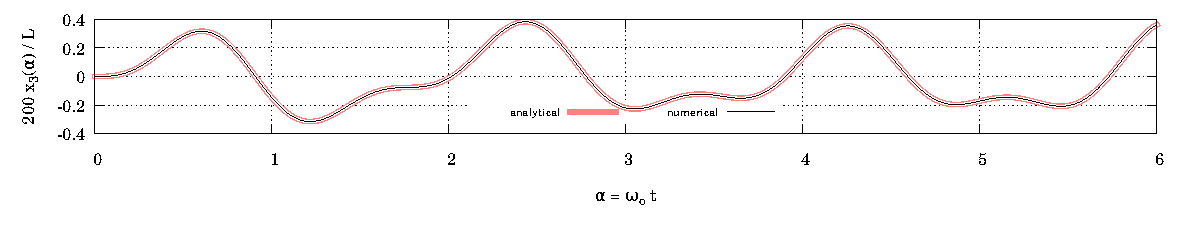
\includegraphics{06/comparison}}%
\end{center}\end{document}
%%% Local Variables: 
%%% mode: latex 
%%% TeX-master: t
%%% End: 
